\documentclass[12pt]{article} 
\usepackage[utf8]{inputenc}
\usepackage{geometry}
\geometry{letterpaper}
\usepackage{graphicx} 
\usepackage{parskip}
\usepackage{booktabs}
\usepackage{array} 
\usepackage{paralist} 
\usepackage{verbatim}
\usepackage{subfig}
\usepackage{fancyhdr}
\usepackage{sectsty}

\pagestyle{fancy}
\renewcommand{\headrulewidth}{0pt} 
\lhead{}\chead{}\rhead{}
\lfoot{}\cfoot{\thepage}\rfoot{}

%%% SECTION TITLE APPEARANCE
\allsectionsfont{\sffamily\mdseries\upshape} 

%%% ToC (table of contents) APPEARANCE
\usepackage[nottoc,notlof,notlot]{tocbibind} 
\usepackage[titles,subfigure]{tocloft}
\renewcommand{\cftsecfont}{\rmfamily\mdseries\upshape}
\renewcommand{\cftsecpagefont}{\rmfamily\mdseries\upshape} %

\usepackage{amsmath}
\usepackage{amssymb}

\title{APMA 0350: Applied Ordinary Differential Equations}
\author{Milan Capoor}
\date{Fall 2022}

\begin{document}
\maketitle
\section{Lecture 1: What is a differential equation?}
\subsection*{Part I - Introduction to the course}
\begin{itemize}
    \item Professor Peyam Tabrizian 
    \item Office Hours Tu 12:15-1:15 pm, Th and F 1:15-2:15
    \item Youtube: https://www.youtube.com/c/DrPeyam/community
\end{itemize}

\subsection*{Part II - What is a Differential equation?}
A differential equation (ODE) is an equation that involves one or more
derivatives of a function y

Examples:
\begin{enumerate}
    \item $y' =2y$ 
    \item $y'' + 5y' + 6y = 0$
    \item $(y''')^2 = \sin (y^3) + y+ t^2$ (where t is independent variable)
    \item $\begin{cases}
        x'(t) = 2x(t) - 3y(t)\\
        y'(t) = 5x(t) + 6y(t)
    \end{cases}$
    \item Partial differential equations (studies in APMA 0360): $\frac{d^2 u}{dx\, dt} + u = \left(\frac{du}{dx}\right)^2$
\end{enumerate}

Applications:
ODEs are used to model and describe many types of processes
\begin{enumerate}
    \item Biology (epidemiology, ecology, cancer research, COVID)
    \item Climate Research (flooding and wildfires)
    \item Economics (stock market, options pricing, wealth and income
    distribution)
    \item Engineering and Physics (from mass-spring systems to aircraft
    design)
    \item Neuroscience and Computer Science (models of brain activity
    patterns, deep learning networks, traffic control)
    \item Modeling outbreak of a Zombie Attack
    \item Chemical Reactions (the PDE that got the PhD!)
\end{enumerate}

From Peyam's PhD advisor:
“If you can solve all differential equations, then you can solve the universe.” $\implies$ DiffEqs are hard to solve but each equation is like its own universe 

\subsection*{Part III - The most basic example}
Example 1: Solve $y' = 2y$ with $y(0) = 3$

Solution:
\begin{enumerate}
    \item Isolate y
    \[y' = 2y \implies \frac{y'}{y} = 2\]

    \item Recognize that the LHS is a derivatives
    \[(\ln |y|)' = 2\]
    \[\ln |y| = 2t + C\]
    \[|y| = e^{2t + C} = e^Ce^{2t}\]
    \[y = \pm e^C e^{2t} = Ce^{2t}\]

    \item Initial condition
    \[y(0) = 3 \implies Ce^0 = 3 \implies C = 3\]
    \[\boxed{y(t) = 3e^{2t}}\]
\end{enumerate}

\textbf{Fact:}
The general solution of $y' = ky$ is 
\[\boxed{y(t) = Ce^{kt}}\]

\subsection*{Part IV - Classification}
\emph{Order:} the highest derivative that appears

Example: 
\begin{enumerate}
    \item $y' = 2y + 1$ is first-Order
    \item $y'' + 5y'+ 6y = 0$ is second-order (second derivative)
    \item $t^5 y''' - 4y' + y = t^3$ is third-order
\end{enumerate}

\emph{Homogeneous:} if the right hand side is 0
\emph{Inhomogeneous:} the right hand is not 0
\begin{enumerate}
    \item $y'' + 5y; + 6y = 0$ is homogeneous
    \item $y'' + 5y' + 6y = t^2$ is inhomogeneous
    \item $y'' + 5y' + 6y + 2t = 2t$ is homogeneous (the 2t terms cancel)
\end{enumerate}

Classifications of ODEs (from easiest to hardest):
\emph{Constant coefficient:}
\begin{enumerate}
    \item $y'' + 5y' + 6y = 0$
    \item $y'' + 5t' + 6y = e^{2t}$
    \item NOT $t^2 y'' + 2y' + 3y = 0$
\end{enumerate}

\emph{Linear DE:} the coefficients can depend on t but not on y
\begin{enumerate}
    \item $y' + ty = 0$
    \item $t^2 y'' + \sin t y' + 2y = 0$
    \item $y'' + 5y' + 6y = 3$
\end{enumerate}

\section{A summary of the first half of the course, the notes for which were lost:}
\subsection*{Lecture Sep 9: Direction Fields}

\emph{Direction field:} A way of qualitatively studying the behaviour of an ODE by plotting the tangent lines at each point. When you draw a line through a point, following the slope arrows, you create a plot of the ODE's solution with that point as the initial condition
- Can be generated with the dfield app (https://aeb019.hosted.uark.edu/dfield.html)

\subsection*{Lecture Sep 12: Qualitative methods}

\emph{Autonomous ODE:} the right-hand-side doesn't depend on t
Special case: Logistic equation $y = \alpha y (1 - \frac{y}{\beta})$
Where $\alpha$ is the growth rate and $\beta$ is the limiting factor. 

\emph{Equilibrium Solutions:} the lines where $f(y) = 0$
To determine what happens at these solutions, we draw a \emph{bifurcation diagram}

For the logistic equation $y= 3y (1 - \frac{y}{20})$, the bifurcation diagram is 

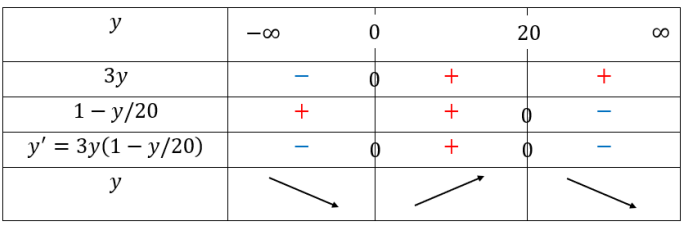
\includegraphics{Images/bifurcation.png}

Which gives us the graph 

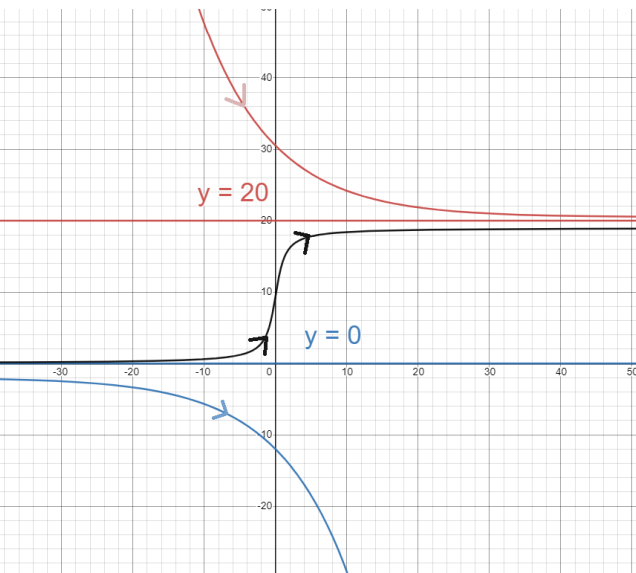
\includegraphics{Images/logistic graph.png}

Classifying solutions:
\begin{itemize}
    \item If the solutions go towards an equilibrium point from each side, it is \emph{stable}
    \item If the solutions move away, it is \emph{unstable}
    \item If the solutions approach from one side and are repelled from the other, it is \emph{bistable}
\end{itemize}

\subsection*{Lecture Sep 14: Existence and uniqueness}
\emph{Existence and Uniqueness Theorem:}
Given $(t_0, y_0)$, consider the ODE 
\[\begin{cases}
    y' = f(y, t)\\
    y(t_0) = y_0
\end{cases}\]
If $f$ and $f_y = \partial f / \partial y$ are continuous near $(t_0, y_0)$, then the ODE has a unique solution $y = y(t)$ for some $t \in (-\delta, \delta), \; \delta > t_0$

Notes:
\begin{itemize}
    \item Because of the uniqueness property, solutions of $y' = f(y, t)$ can never cross
    \item If you only want \emph{existence}, it is enough to assume that $f$ is continuous (you don't need the partial derivative!) 
\end{itemize}

\subsection*{Lecture Sep 16: Separable Equations}
\emph{Separable equation:} an equation in the form 
\[y' = \frac{f(t)}{g(y)}\]

Example 1:
\[\begin{cases}
    t^2 \left(\frac{dy}{dt}\right) = (1 -t^2)(y^2 + 1)\\
    y(1) = 0
\end{cases}\]

Solution:
\[\frac{1}{y^2 + 1} \; dy = \frac{1 - t^2}{t^2} \; dt\]
\[\int \frac{1}{y^2 + 1} \; dy = \int \frac{1}{t^2} - 1 \; dt\]
\[\tan^{-1} y = -\frac{1}{t} - t + C\]
\[y = \tan \left(-\frac{1}{t} - t + C\right)\]
\[0 = \tan (-1 - 1 + C) implies C = 2\]
\[\boxed{y = \tan \left(-\frac{1}{t} - t + 2\right)}\]

Example 2: Solving the logistic equation
\[\begin{cases}
    y' = 3y\left(1 - \frac{y}{20}\right)\\
    y(0) = 10
\end{cases}\]

Solution:
\[\frac{dy}{y (1 - \frac{y}{20})} = 3\; dt\]
\[\int \frac{dy}{y (\frac{20 - y}{20})} = \int 3 \; dt\]
\[\int \frac{20}{y(20 - y)}\; dy = 3t + C\]

To evaluate the left hand side, we must use \emph{partial fractions}:
\[\frac{20}{y(20 - y)} = \frac{A}{y} + \frac{B}{20 - y} = \frac{20A - Ay + By}{y(20 - y)} = \frac{20A + (B - A)y}{y(20 - y)}\]
\[20 = 20A + (B - A)y\]
\[\begin{cases}
    20A = 20\\
    (B - A) = 0
\end{cases} \implies \begin{cases}
    A = 1\\
    B = 1
\end{cases}\]
\[\implies \frac{20}{y (20 - y)} = \frac{1}{y} + \frac{1}{20 - y}\]

Going back to the problem above:
\[\int \frac{20}{y(20 - y)}\; dy = 3t + C\]
\[\int \frac{1}{y} + \frac{1}{20 - y}\; dy = 3t + C\]
\[\ln |y| - \ln |20 - y| = 3t + C\]
\[\ln \left|\frac{y}{20 - y}\right| = 3t + C\]
\[\frac{y}{20 - y} = \pm e^C e^{3t}\]
\[y = Ce^{3t} (20 - y) = 20Ce^{3t} - Cye^{3t}\]
\[y(1 + Ce^{3t}) = 20Ce^{3t}\]
\[\boxed{y = \frac{20Ce^{3t}}{1 + Ce^{3t}}}\]

\subsection*{Lecture Sep 19: Integrating Factors}
To solve equations in the form
\[y' + \alpha y = f(t)\]
multiply by $e^{at}$

Example 1: 
\[\begin{cases}
    3y' = 6y + t\\
    y(0) = 1
\end{cases}\]

Solution:
\[3y' - 6y = t\]
\[y' - 2y = \frac{1}{3}t\]
\[(y' - 2y)e^{-2t} = \frac{1}{3}te^{-2t}\]
\[y'e^{-2t} - 2y e^{-2t} = \frac{1}{3}te^{-2t} \]
\[(y e^{-2t})' = \frac{1}{3}te^{-2t}\]
\[y e^{-2t} = \int \frac{t}{3}e^{-2t}\]
\[y e^{-2t} = \frac{t}{3} \frac{e^{-2t}}{-2} - \int \frac{1}{3} \frac{e^{-2t}}{-2}\; dt \quad \text{(By parts)}\]
\[y e^{-2t} = -\frac{te^{-2t}}{6} - \frac{1}{12}e^{-2t}+C\]
\[\boxed{y = -\frac{t}{6} - \frac{1}{12} + Ce^{2t}}\]

\emph{More general integrating factor:}
For \[y' + P(t) y = f(t)\]
multiply by 
\[e^{\int P(t) dt}\]

Example 2: 
\[y' + 3t^2 y = 6t^2\]

Solution:
\[(y e^{\int 3t^2\; dt})'= 6t^2 e^{\int 3t^2\; dt}\]
\[(y e^{t^3})' = 6t^2 e^{t^3}\]
\[ye^{t^3} = \int 6t^2 e^{t^3} \; dt \quad (u = t^3, 2du = 6t^2\; dt)\]
\[ye^{t^3} = \int 2e^u \; du = 2e^u + C = 2e^{t^3} + C\]
\[y = 2 + Ce^{-t^3}\]

\subsection*{Lecture Sep 21: Exact Equations}
\emph{Exact equation:} equation in the form 
\[P(x, y) \; dx + Q(x, y) \; dy\]

Many ODEs can be reduced to this form:
\[y' = \frac{2xy + y^2}{x^2 + 2xy}\]
\[\implies (x^2 + 2xy) \; dy = -(2xy + y^2) \; dx\]
\[\implies (x^2 + 2xy) \; dy + (2xy + y^2) \; dx = 0\]

Notice, this is the same notation used to solve line integrals in Multivariable calculus!

\emph{Gradient:} If $f = f(x,y)$, then $\nabla f = \langle f_x, f_y \rangle$

To solve, we must find a \emph{potential function} $f$ of $F(x, y)$ such that $F = \nabla f$

Example 1: Find f for $F(x,y) = \langle2xy + y^2, x^2 + 2xy\rangle$
Solution:
\begin{enumerate}
    \item Check that F is conservative
    \[P_y = 2x + 2y\]
    \[Q_x = 2x + 2y\]
    \[P_y = Q_x, \; \therefore F \text{ is conservative}\]
    Because F is conservative, a potential function exists 

    \item Find $f$
    \[F = \nabla f \implies \langle P, Q\rangle = \langle f_x, f_y \rangle\]
    \[f_x = 2xy + y^2 \implies f = \int 2xy + y^2\; dx = x^2y + y^2x + g(y)\]
    \[f_y = x^2 + 2xy \implies f = \int x^2 + 2xy\; dy = x^2 y + xy^2 + f(x)\]

    Collecting all the terms,
    \[f(x, y) = x^2 y + xy^2\]
\end{enumerate}

Amazingly for an ODE 
\[P\; dx = Q\; dy = 0, \quad F = \langle P, Q \rangle\]
the solution is just 
\[f(x, y) = C\]

Therefore, for the example above 
\[x^2y + xy^2 = C\]
(in implicit form)

\emph{Non-exact equations:}
Example 2: $(3xy + y^2) \; dx + (x^2 + xy) \; dy = 0$

Solution:
\[P_y = 3x + 2y\]
\[Q_x = 2x + y\]
So the equation is not exact!

But, we can multiply the ODE by $x$ to get 
\[(3x^2 y + xy^2) \; dx + (x^3 + x^2 y) \; dy = 0\]

In practice, this integrating factor is very difficult to find (requires PDEs) so will be given in this course where necessary. 

Here,
\[P_y = 3x^2 + 2xy\]
\[Q_x = 3x^2 + 2xy\]
\[P_y = Q_x\]

\[f_x = 3x^2 y + xy^2 \implies f = \int 3x^2 y + xy^2 \; dx = x^3 y + \frac{1}{2}x^2 y^2 + g(y)\]
\[f_y = x^3 + x^2 y \implies f = \int x^3 + x^2 y \; dy = x^3 y + x^2 \frac{y^2}{2} + g(x)\]
\[f(x, y) = x^3 y + \frac{1}{2}x^2 y^2\]

Therefore, 
\[\boxed{x^3 y + \frac{1}{2}x^2 y^2 = C}\]

\subsection*{Lecture Sep 28: Numerical Methods I}
\emph{Euler's Method:}
\[y_{n + 1} \approx y_n + h f(y_n, t_n)\]

Given an ODE $y' = f(y, t)$, an initial condition $(t_0, y_0)$, and a number of steps $N$, we can approximate the value of the function at a point by applying the above equation where the step size is  
\[h = \frac{t_n - t_0}{N}\] 

Example 1: Find an approximation of $y(2)$ where 
\[\begin{cases}
    y' = y^2 + 3t\\
    y(0) = 2
\end{cases}\]

Solution:
\[h = \frac{2 - 0}{2} = 1\]
\begin{align*}
    y_0 &= 2\\
    y_1 &= y(0) + f'(2, 0) = 2 + 4 = 6\\
    y_2 &= y(1) + f'(6, 1) = 6 + 39 = 45
\end{align*}

The smaller and more numerous the steps, the more accurate the approximation. 

Indeed, this can be automated via Python computation. 

\subsection*{Lecture Sep 30: Numerical Methods II}
While often good for basic approximations, Euler's method has a number of drawbacks:
\begin{enumerate}
    \item Sensitivity to initial conditions (if there is an exponential term and an issue with rounding, the solution can explode)
    \item Instability (you may need a very small h value to accurately plot a solution, particularly when solutions oscillate)
\end{enumerate}

Alternatives to Euler's method: 
\begin{enumerate}
    \item Backwards Euler:
    \[y_{n+1} = y_n + hf(t_{n + 1}, y_{n + 1})\]
    This is an implicit method that requires knowledge of $y_{n + 1}$

    \item Multistep method 
    \[y_{n+1} = y_n \frac{3}{2}hf(t_n, y_n) - \frac{1}{2}hf(t_{n - 1}, y_{n -1})\] 

    Uses both present and past values of y

    \item Runge-Kutta 
    \[y_{n+ 1} = y_n + hf(t_n + \frac{h}{2}, \; y_n + \frac{h}{2} f(t_n, y_n))\]
    More complicated, but evaluates f at multiple points resolving all other issues
\end{enumerate}

ODEs can also be solved symbolically in Python with the dsolve library in Sympy.

\subsection*{Lecture Oct 3: Systems of ODE I}
Many interactions between objects can be modelled as systems of ODEs which we can represent as matrix equations in the form $\vec{x}' = A\vec{x} + \vec{f}$.

Example 1: 
\[\begin{cases}
    x_1'(t) = 7x_1(t) + 2x_2(t) + t^2\\
    x_2'(t) = -4x_1(t) + x_2(t)
\end{cases}\]
\[\implies \begin{bmatrix}
    x_1'\\
    x_2'
\end{bmatrix} = \begin{bmatrix}
    7 & 2\\
    -4 & 1
\end{bmatrix} \begin{bmatrix}
    x_1\\
    x_2
\end{bmatrix} + \begin{bmatrix}
    t^2\\
    0
\end{bmatrix}\]

\emph{Higher order equations:} Moreover, we can turn any higher order ODE into a system 

Example 2: $y'' + 4y = 0$
Solution:
\[x_1(t) = y, \quad x_2(t) = y'\]
\[\begin{cases}
    x_1' = y' = x_2\\
    x_2' = y'' = -4y = -4x_1
\end{cases}\]
\[\begin{cases}
    x_1' = 0x_1 + x_2\\
    x_2' = -4x_1 + 0x_2
\end{cases}\]
\[\vec{x}(t) = \begin{bmatrix}
    0 & 1\\
    -4 & 0
\end{bmatrix} \vec{x}(t)\]

\subsection*{Lecture Oct 5: Linear Algebra Review}
If for some vector $\vec{v}$, a matrix A, and a scalar value $\lambda$, 
\[A\vec{v} = \lambda\vec{v}\]
then,
$\lambda$ is an \emph{eigenvalue} of A and $\vec{v}$ is an \emph{eigenvector} of A corresponding to $\lambda$

If $\vec{v}$ is an eigenvector, $A\vec{v}$ will lie in its span. 

To find an eigenvalue, solve the equation
\[\det (A - \lambda I) = 0\]

To find the eigenvectors, find the nullspace of $A - \lambda I$: 
\[(A - \lambda I)\vec{v} = \vec{0}\]

\emph{Diagonalization:} a matrix A can be written in the form $A = PDP^{-1}$ where
\[D = \begin{bmatrix}
    \lambda_1 & 0\\
    0 & \lambda_2
\end{bmatrix}, \quad P = \begin{bmatrix}
    \vec{v}_1 & \vec{v}_2
\end{bmatrix}\]\

\subsection*{Systems of ODE II}
The solution of an equation in the form $x' = Ax$ is 
\[x(t) = C_1 \, e^{\lambda_1 t}\; \vec{v}_{\lambda_1} + C_2 \, e^{\lambda_2 t}\; \vec{v}_{\lambda_1}\]

Example 1: Solve $x' = \begin{bmatrix}
    7 & -3\\
    10 & -4
\end{bmatrix}$

Eigenvalues:
\[\begin{vmatrix}
    7 - \lambda & -3\\
    10 & -4 - \lambda
\end{vmatrix} = (7- \lambda)(-4-\lambda) +30 = \lambda^2 - 3\lambda + 2\]
\[(\lambda - 2)(\lambda - 1) = 0 \implies \lambda = \{1, 2\}\]

Eigenvector for $\lambda = 1$:
\[\begin{array}{c c | c}
    6 & -3 & 0\\
    10 & -5 & 0
\end{array} \implies 2x_1 - x_2 = 0\]
\[\vec{v}_{\lambda = 1} = \begin{bmatrix}
    1\\
    2
\end{bmatrix}\]

Eigenvector for $\lambda = 2$:
\[\begin{array}{c c | c}
    5 & -3 & 0\\
    10 & -6 & 0
\end{array} \implies 5x_1 - 3x_2 = 0\]
\[\vec{v}_{\lambda = 2} = \begin{bmatrix}
    3\\
    5
\end{bmatrix}\]

Solution:
\[\boxed{x(t) = C_1 e^{t} \begin{bmatrix}
    1\\2
\end{bmatrix} + C_2 e^{2t} \begin{bmatrix}
    3\\5
\end{bmatrix}}\]

\emph{Phase portraits:}
To draw a phase portrait, solve the system and plot the axes determined by the eigenvectors. On each eigenvector, draw an arrow in the direction of the sign of the eigenvalue for that eigenvector (outwards if positive, inwards if negative). Then, sketch the solutions by drawing lines between the axes according to those arrows.

Example 2: Draw the phase portrait for the curve 
\[x(t) = C_1 e^{-2t} \begin{bmatrix}
    1\\-1
\end{bmatrix}+ C_2 e^{4t} \begin{bmatrix}
    1\\1
\end{bmatrix}\]

Solution:

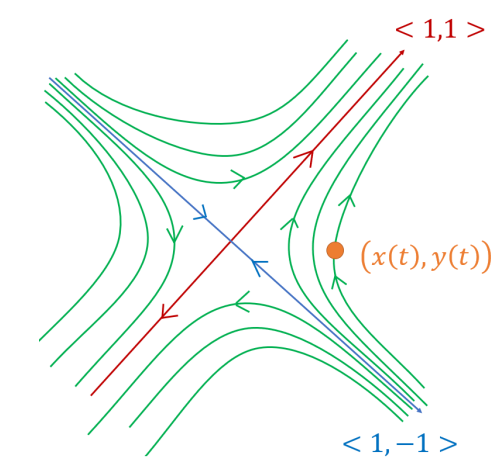
\includegraphics{Images/phase portrait.png}

\subsection*{Oct 12: Complex Eigenvalues}
Remember:
\[i = \sqrt{-1}\]
\[e^{it} = \cos t + i \sin t\]

To solve a system with complex eigenvalues, we need to find a generalized eigenvector. 

Example 1: $x' = \begin{bmatrix}
    -2 & 4\\
    -2 & 2
\end{bmatrix} x$

Here, $\lambda = \pm 2i$

Eigenvector for $\lambda = 2i$:
\[\text{Nul}(A- (2i)I) - \begin{array}{c c | c}
    1 + i & -2 & 0\\
    1 & -1 + i & 0
\end{array}\]
Trick: because we know that $2i$ is an eigenvalue, one of the two rows has to be 0. Choose one and set the other to 0. 
\[\implies \begin{array}{c c | c}
    1 + i & -2 & 0\\
    0 & 0 & 0
\end{array} \implies (1+ i)x_1 -2x_2 = 0\]
\[\vec{v}_{\lambda = 2i} = \begin{bmatrix}
    2\\
    1 + i
\end{bmatrix}\]

Because of the rules of complex conjugates, we don't need the other eigenvector!

Instead, we know that 
\[e^{(2i) t} \begin{bmatrix}
    2\\ 1 +i
\end{bmatrix}\]
is a solution. As we are looking for real solutions, we can use Euler's identity:

\[e^{(2i) t} \begin{bmatrix}
    2\\ 1 +i
\end{bmatrix} = \left(\cos(2t) + i \sin(2t)\right)\left(\begin{bmatrix}
    2\\1
\end{bmatrix} + i \begin{bmatrix}
    0\\1
\end{bmatrix}\right)\]
\[= \left(\cos(2t) \begin{bmatrix}
    2\\1
\end{bmatrix} - \sin(2t) \begin{bmatrix}
    0\\1
\end{bmatrix}\right) + i \left(\cos (2t) \begin{bmatrix}
    0\\1
\end{bmatrix} + \sin(2t) \begin{bmatrix}
    2\\1
\end{bmatrix}\right)\]

So the general solution is 
\[\boxed{x(t) = C_1 \begin{bmatrix}
    2\cos (2t)\\
    \cos(2t) - \sin (2t)
\end{bmatrix} + C_2 \begin{bmatrix}
    2 \sin (2t)\\
    \cos(2t) + \sin(2t)
\end{bmatrix}}\]

To draw a phase portrait, use the principal part of the eigenvector. DO NOT use the generalized eigenvector. The cos and sin terms will then create some kind of elliptical shape where the argument to the trig functions determines if the solution flows clockwise or counterclockwise. 

\subsection*{Lecture Oct 14: Repeated Eigenvalues}
In the case of a single, repeated eigenvalue, find the first eigenvector as normal and then row reduce with that value to find the general. Then, in the final solution, add a correcting factor (which will become clear after studying 2nd order ODEs).

Example 1: $x' - \begin{bmatrix}
    1 & 1\\
    -1 & 3
\end{bmatrix}$

Eigenvalue:
\[\begin{vmatrix}
    1 - \lambda & 1\\
    -1 & 3 - \lambda
\end{vmatrix} = (1 - \lambda)(3 - \lambda) + 1 = \lambda^2 -4\lambda + 4\]
\[(\lambda - 2)^2 = 0 \implies \lambda = 2\]

Eigenvector for $\lambda = 2$:
\[\begin{array}{c c | c}
    -1 & 1 & 0\\
    -1 & 1 & 0
\end{array} \implies -x_1 + x_2 = 0\]
\[\vec{v}_{\lambda = 2} = \begin{bmatrix}
    1\\1
\end{bmatrix}\]

Generalized eigenvector:
\[(A - 2I)\vec{w} = \begin{bmatrix}
    1\\1
\end{bmatrix}\]
\[\begin{array}{c c |c}
    -1 & 1 & 1\\
    -1 & 1 & 1
\end{array} \implies -x_1 + x_2 = 1\]
\[y = 1 + x\]
\[\vec{x} = \begin{bmatrix}
    x\\
    1 + x
\end{bmatrix} = x \begin{bmatrix}
    1\\1
\end{bmatrix} + \begin{bmatrix}
    0\\1
\end{bmatrix}\]

Solution:
\[\boxed{x(t) = C_1 e^{2t} \begin{bmatrix}
    1\\1
\end{bmatrix} + C_2\left(te^{2t} \begin{bmatrix}
    1\\1
\end{bmatrix} + e^{2t} \begin{bmatrix}
    0\\1
\end{bmatrix}\right)}\]

Note: you are not allowed to rescale the generalized eigenvector

\emph{Plotting phase portraits:} Just like direction fields, phase portraits can be created with a helpful computer program: pplane (https://aeb019.hosted.uark.edu/pplane.html).

Note: when inputting equations into pplane, all multiplications must be explicit (e.g. 3*x not 3x) and no spaces are allowed (e.g. 3+x not 3 + x)

\subsection*{Oct 17: Matrix exponentials}
Notice that equations in the form $x' = Ax$ is analgous to the elementary equation $y' = \alpha y \implies y = Ce^{\alpha t}$. 

Thus, to solve a matrix equation we \emph{can} say that 
\[x = Ce^{At} = Pe^{Dt}P^{-1} \begin{bmatrix}
    C_1\\
    C_2
\end{bmatrix}\]
by the properties of diagonal matrices. 

Example 1: Solve $x' = \begin{bmatrix}
    0 & 1\\
    -2 & 3
\end{bmatrix}$

Eigenvalues:
\[\begin{vmatrix}
    -\lambda & 1\\
    -2 & 3 - \lambda
\end{vmatrix} = \lambda^2 - 3\lambda + 2 = 0\]
\[(\lambda - 1)(\lambda - 2) = 0 \implies \lambda = \{1, 2\}\]

Eigenvector for $\lambda = 1$:
\[\begin{array}{c c |c}
    -1 & 1 & 0\\
    -2 & 2 & 0
\end{array} \implies -x_1 + x_2 = 0\]
\[\vec{v}_{\lambda = 1} = \begin{bmatrix}
    1\\
    1
\end{bmatrix}\]

Eigenvector for $\lambda = 2$:
\[\begin{array}{c c |c}
    -2 & 1 & 0\\
    -2 & 1 & 0
\end{array} \implies -2x_1 + x_1 = 0\]
\[\vec{v}_{\lambda = 2} = \begin{bmatrix}
    1\\
    2
\end{bmatrix}\]

Solution:
\[e^{At} = pe^{Dt}P^{-1}\]
\[ = \begin{bmatrix}
    1 & 1\\
    1 & 2
\end{bmatrix} \begin{bmatrix}
    e^t & 0\\
    0 & e^{2t}
\end{bmatrix} \begin{bmatrix}
    1 & 1\\
    1 & 2
\end{bmatrix}^{-1}\]
\[= \begin{bmatrix}
    2e^t - e^{2t} & -e^t + e^{2t}\\
    2e^t - 2e^{2t} & -e^t + 2e^{2t}
\end{bmatrix}\]

\[\boxed{x(t) = C_1 \begin{bmatrix}
    2e^t - e^{2t}\\
    2e^t - 2e^{2t}
\end{bmatrix} + C_2 \begin{bmatrix}
    -e^t + e^{2t}\\
    -e^t + 2e^{2t}
\end{bmatrix}}\]

\emph{Matrix exponentials with repeated eigenvalues:}
For $2 \times 2$ matrices with one eigenvalue 
\[(A - \lambda I)^2 = 0\]

So, when calculating the Taylor expansion of a matrix exponentiation, all higher terms go to 0. 

So, 
\[e^{At} = e^{\lambda t}e^{(A - \lambda I) t} = e^{\lambda t} \left(I + (A - \lambda I)t\right)\]

Example 2: Solve $x' = \begin{bmatrix}
    -3 & -1\\
    1 & -5
\end{bmatrix}x$

Eigenvalues:
\[\begin{vmatrix}
    -3 - \lambda & -1\\
    1 & -5 - \lambda
\end{vmatrix} = \lambda^2 + 8\lambda + 16\]
\[(\lambda + 4)^2 = 0 \implies \lambda = -4\]

\[e^{At} = e^{-4t}\left(\begin{bmatrix}
    1 & 0\\
    0 & 1
\end{bmatrix} + t\begin{bmatrix}
    1 & -1\\
    1 & -1
\end{bmatrix}\right)\]
\[= e^{-4t} \begin{bmatrix}
    1 + t & -t\\
    t & 1 -t
\end{bmatrix}\]

\[\boxed{x(t) = C_1 e^{-4t} \begin{bmatrix}
    1 + t\\
    t
\end{bmatrix} + C_2 e^{-4t} \begin{bmatrix}
    -t \\
    1- t
\end{bmatrix}}\]

\subsection*{Lecture Oct 19: Nonlinear systems}
For a nonlinear system of interacting $x'$ and $y'$ equations, we can express the system in a form $\vec{x}'(t) = F(\vec{x}(t))$ where:
\[\vec{x}(t) = \begin{bmatrix}
    x(t)\\
    y(t)
\end{bmatrix}, \quad F(x, y) = \begin{bmatrix}
    x'\\
    y'
\end{bmatrix}\]

Recalling the existence-uniqueness theorem, this system will have a unique solution if F and $\nabla F$ are continuous where 
\[\nabla F = \begin{bmatrix}
    \frac{\partial x'}{\partial x} & \frac{\partial x'}{\partial y}\\
    \frac{\partial y'}{\partial x} & \frac{\partial y'}{\partial y}
\end{bmatrix}\]

Example 1: Determine whether a solution exists for 
\[\begin{cases}
    x' = x^2 + xy + e^y\\
    y' = \cos x + 2y
\end{cases}\]

\[F(x, y) = \begin{bmatrix}
    x^2 + xy + e^y\\
    \cos x + 2y
\end{bmatrix}\]
\[\nabla F = \begin{bmatrix}
    2x + y & x + e^y\\
    -\sin x & 2
\end{bmatrix}\]

All these entries are continuous so the ODE has a unique solution for $t$ close enough to 0.

\emph{Classifying equilibrium solutions:}
To classify equilibria, we need to find the linearized systems ($\vec{x}' = \nabla F(\vec{x})$) at those points. To achieve this classification, simply find the eigenvalues of the jacobian at that point.

Example 2: Classify the equilibria of 
\[\begin{cases}
    x' = -x + xy\\
    y' = -8y + 4xy
\end{cases}\]

Solution:
\begin{enumerate}
    \item Find the nullclines 
    \[\begin{cases}
        -x + xy = 0\\
        -8y + 4xy = 0
    \end{cases} \implies \begin{cases}
        x = 0 \text{ or } y = 1\\
        y = 0 \text{ or } x = 2
    \end{cases} \implies (0, 0) \text{ and } (2, 1)\]

    \item Find the linearization
    \[\nabla F = \begin{bmatrix}
        -1 + y & x\\
        4y & -8 + 4x
    \end{bmatrix}\]

    \item Check (0, 0)
    \[\nabla F(0, 0) = \begin{bmatrix}
        -1 & 0\\
        0 & -8
    \end{bmatrix} \implies \lambda = \{-1, -8\}\] 
    So the point (0, 0) is a sink (both are negative)

    \item (This problem finished in the next section)
\end{enumerate}

\section{Lecture: Oct 21}
\subsection*{Part I - Classifying Equilibrium Points of Nonlinear ODEs}
Example 1: Classify the equilibrium points of
\[\begin{cases}
    x' = -x + xy\\
    y' = -8y + 4xy
\end{cases}\]

To find the equilibrium points, set $x' = 0$ and $y' = 0$

In this equation,
\[\begin{cases}
    x' = -x(1 - y) = 0\\
    y' = -y(8 - 4x) = 0
\end{cases} \implies (0, 0) \quad (2, 1)\]

Linearization:
\[\nabla F(x, y) = \begin{bmatrix}
    \frac{\partial (-x + xy)}{\partial x} & \frac{\partial (-x + xy)}{\partial y}\\
    \frac{\partial (-8y + 4xy)}{\partial x} & \frac{\partial (-8y + 4xy)}{\partial y}\\
\end{bmatrix} = \begin{bmatrix}
    -1 + y & x\\
    4y & -8 + 4x
\end{bmatrix}\]

Case 1: $(0, 0)$
\[\nabla F(0, 0) = \begin{bmatrix}
    -1 & 0\\
    0 & -8
\end{bmatrix}\]

The eigenvalues of this are $\lambda = -1$ and $\lambda = - 8$, both of which are less than zero so the solution is a sink and the point $(0, 0)$ is \textbf{stable}.

Note: For a complex negative eigenvalue (e.g. $\lambda = -2 + 3i$), there will be a spiral sink which is also stable

Case 2: $(2, 1)$
\[\nabla F(2, 1) = \begin{bmatrix}
    0 & 2\\
    4 & 0
\end{bmatrix}\]

Eigenvalues:
\[\lambda^2 - 8 = 0 \implies \lambda = \pm 2\sqrt{2}\]

In this case, one eigenvalue is positive and the other is negative so this is a \textbf{semi-stable saddle point}

Stability cases summary:
\begin{itemize}
    \item If the eigenvalues are both negative, we have a sink
    \item If both positive, unstable
    \item If one positive and one negative, saddle point
    \item If 0, "screwed"
\end{itemize}

\subsection*{Part II - Application Number 1: Competing Species}
Recall: Logistic equation 
\[y' = 3t \left(1 - \frac{y}{20}\right)\]
(the growth of a population with limited resources, where 3 is the growth rate and 20 is the limiting factor)

Guiding question: What if you have two coexisting animal species?
\[\begin{cases}
    x(t) = \text{ population of rabbits}\\
    y(t) = \text{ population of sheep}\\
\end{cases}\]

Note: The two species do not prey on each other but compete for the same limited resources 

\begin{enumerate}
    \item Logistic Approach:
    \[\begin{cases}
        x' = 3x(1 - \frac{x}{1.5})\\
        y' = 2y(1 - \frac{y}{2})
    \end{cases} = \begin{cases}
        x' = 3x - 2x^2\\
        y' = 2y - y^2
    \end{cases}\]
    
    However, this model does not account for competition for limited resources
    
    \item A better model!
    \[\begin{cases}
        x' = 3x - 2x^2 - xy\\
        y' = 2y - y^2 - xy
    \end{cases}\]
    Here, the xy term accounts for the interaction between the two populations 
    (if either were 0, the term would go to zero)
\end{enumerate}

\subsection*{Part III - Equilibria}
Example 2: Find the equilibrium points of the model 
\[\begin{cases}
    x' = x(3 - 2x - y) = 0\\
    y' = y(2 - y - x) = 0
\end{cases}\]

\[\begin{cases}
    x = 0 \implies y = \{0, 2\} \implies \boxed{(0, 0) \quad (0, 2)}\\
    3 - 2x - y = 0 \implies (y = 0 \implies x = \frac{3}{2}) \\
    \text{ OR } \left(2-y-x = 0 \implies \begin{cases}
        3 - 2x - y = 0\\
        2 - y - x = 0
    \end{cases} \implies x = 1, \quad y = 1\right) \implies \boxed{(\frac{3}{2}, 0) \quad (1, 1)}
\end{cases}\]

Thus, the four possible outcomes:
\begin{enumerate}
    \item $(0, 0)$ - Both die 
    \item $(0, 2)$ - Sheep win
    \item $(\frac{3}{2}, 0)$ - Bunnies win 
    \item $(1, 1)$ - Coexistence
\end{enumerate}

To classify each point, we use the linearization:
\[\nabla F(x, y) = \begin{bmatrix}
    \frac{\partial (3x - 2x^2 0 xy)}{\partial x} & \frac{\partial (3x - 2x^2 0 xy)}{\partial y}\\
    \frac{\partial (2y - y^2 - xy)}{\partial x} & \frac{\partial (2y- y^2 - xy)}{\partial y}
\end{bmatrix} = \begin{bmatrix}
    3 - 4x - y & -x\\
    -y & 2 - 2y - x
\end{bmatrix}\]

Thus,
\begin{enumerate}
    \item $F(0, 0) = \begin{bmatrix}
        3 & 0 \\
        0 & 2
    \end{bmatrix} \implies \lambda = \{3, 2\} \implies$ the system is unstable 
    \item $F(0, 2) = \begin{bmatrix}
        1 & 0\\
        -2 & -2
    \end{bmatrix} = \lambda = \{1, -2\} \implies$ the system is semistable so the sheep will survive
    \item $F(\frac{3}{2}, 0) = \begin{bmatrix}
        -3 & -\frac{3}{2}\\
        0 & \frac{1}{2}
    \end{bmatrix} \implies \lambda = \{-3, \frac{1}{2}\} \implies $ the system is also a saddle so the bunnies survive
\end{enumerate}

\section{Lecture: Oct 24}
\subsection*{Part I - Rabbits and Sheep Model Recap}
Our model, where x is the population of rabbits and y is the population of sheep:
\[\begin{cases}
    x' = 3x - 2x^2 - xy\\
    y' = 2y - y^2 - xy
\end{cases}\]

Equilibrium points: $(0, 0), \; (0, 2), \; (\frac{3}{2}, 0),\; (1, 1)$

\subsection*{Part II - Classification continued}
\[\nabla F(x, y) = \begin{bmatrix}
    3 - 4x - y & -x\\
    -y & 2 - 2y - x
\end{bmatrix}\]
"Again, this is applied math. There is no reason we add this term. It just works. And if it doesn't, we work harder and make up a different term that just works"

\[\nabla F(1, 1) = \begin{bmatrix}
    -2 & -1\\
    -1 & -1
\end{bmatrix}\] 

Eigenvalues:
\[| A - \lambda I | = (-2 - \lambda)(-1 - \lambda) - 1 = \lambda^2 + 3 \lambda + 1 = 0\]
\[\lambda = \frac{-3 \pm \sqrt{9 - 4(1)}}{2} = -\frac{3}{2} \pm \frac{\sqrt{5}}{2}\]

Here, both eigenvalues are negative so (1, 1) is stable

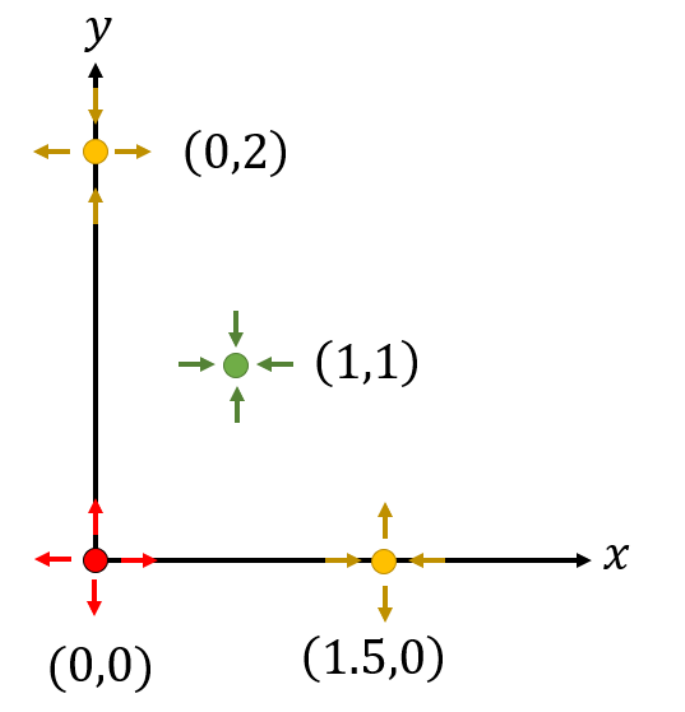
\includegraphics{Images/rabbits and bunnies plot.png}

Note: We do not know which directions of the saddle are positive and which are negative

To draw the rest of the picture, we need to the region $x \in [0, \frac{3}{2}]$ and $y \in [0, 2]$ because those coordinates are the limiting factors of the system 

\subsection*{Part III - Nullclines}
We want to study the behavior of solutions on the axes $x = 0, y = 0, x = 1.5, y = 2$

\emph{Nullclines:} axes where x' or y' is 0

\begin{itemize}
    \item Case 1: $x = 0$ (no rabbits)
        \[\begin{cases}
            x' = 0\\
            y' = 2y - y^2
        \end{cases}\]
        As a result, we are only concerned with vertical movement on the axis.

        Looking at the sign of y', we see that it will be positive $[0, 2]$ and negative $[2, \infty]$

        Therefore, the arrows will be moving up on the y-axis up to 2 and decreasing above 2, so we also now know the orientation of the saddle point.

        Interpretation: if there are no rabbits, the population of sheep will simply increase until they hit their own carrying capacity (which is exactly what we expect!)

    \item Case 2: $y = 0$ (no sheep)
    \[\begin{cases}
        x' = 3x - 2x^2\\
        y' = 0
    \end{cases}\]
    So x will increase until it reaches $x = \frac{3}{2}$

    \item Case 3: $y = 2$ (sheep reached limiting pop)
        \[\begin{cases}
            x' = x - 2x^2\\
            y' = -2x
        \end{cases}\]

        The sign of y' is negative, so on this axis the arrows are pointing down. And, because x' is positive $[0, \frac{1}{2}]$ and negative $[\frac{1}{2}, 1.5]$, the arrows also point roughly towards the centre of the region 

    \item Case 4: $x = 1.5$ (saddle)
        \[\begin{cases}
            x' = - \frac{3}{2}y\\
            y' = \frac{1}{2}y - y^2
        \end{cases}\]

        The sign of x' is negative so the arrows point to the left, and y' is positive on $[0, \frac{1}{2}]$ and negative $[\frac{1}{2}, 2]$
\end{itemize}

From all of this, we can fill in the graph from earlier and draw a few solutions:

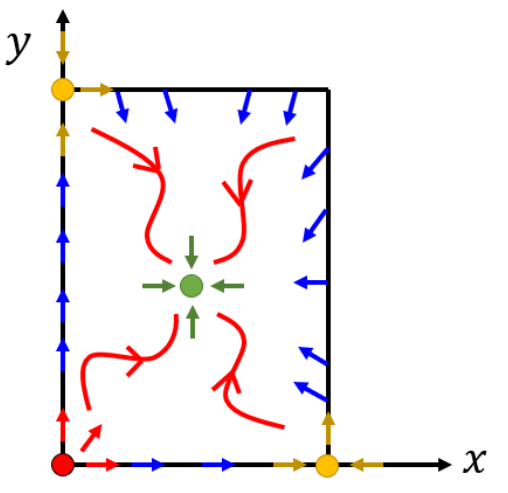
\includegraphics{Images/rabbits and bunnies plot 2.png}

Epic conclusion: the species will not go extinct! they will happily coexist and eventually reach the equilibrium (1, 1)

BUT: we missed the case where there is a periodic orbit around the equilibrium point and where the two species struggle for eternity

\subsection*{Part IV - Periodic Orbits}
To rule out the possibility of periodic orbits, we just need to examine the behavior of the system at the axes of the equilibrium point.

\begin{itemize}
    \item Case 1: $x = 1$
    \[\begin{cases}
        x' = 2x - 2x^2\\
        y' = 1 - x
    \end{cases}\]

    So on the axis $y = 1$, if $x < 1$, the arrows are pointing up, and if $x > 1$, they are pointing down.

    \item Case 2: $y = 1$
    \[\begin{cases}
        x' = 1 -y\\
        y' = -y + y^2
    \end{cases}\]
    So on the axis x = 1, if y < 1, the arrows are pointing to the right (increasing) and if y > 1, they are pointing to the left (x decreasing)
\end{itemize}

Completing the picture, we see that no periodic orbit is possible!

\section{Lecture: Oct 26}
\subsection*{Part I - Chemical Tanks}
Assume there are three chemical tanks in series.
\begin{itemize}
    \item Tank 1: $Q_1(t)$ kg salt, 2L water
    \item Tank 2: $Q_2(t)$ kg salt, 4L water
    \item Tank 3: $Q_3(t)$ kg, 3L water
    \item The first tank has an input of 6L/min of water and 1/3 kg/L salt 
    \item Each minute, 4L salinated water flows from the first tank to the second and from the second to the third
    \item The third tank has an output of 12 L/min
\end{itemize}

Set up a system in the form $Q'(t) = AQ(t) + b$

\begin{enumerate}
    \item $Q'_1(t) = 6 (\frac{1}{3}) - 4 \left(\frac{Q_1(t)}{2}\right) = 2 - 2 Q_1(t)$
    \item $Q_2'(t) = 4 \left(\frac{Q_1(t)}{2}\right) - 4\left(\frac{Q_2(t)}{4}\right) = 2Q_1(t) - Q_2(t)$
    \item $Q_3'(t) = 4\left(\frac{Q_2(t)}{4}\right) - 12\left(\frac{Q_2(t)}{3}\right) = Q_2(t) - 4Q_3(t)$
\end{enumerate}

So, the system is 
\[\begin{cases}
    Q_1' = -2Q_1 + 2\\
    Q_2' = 2Q_1 - Q_2
    Q_3' = Q_2 - 4Q_3
\end{cases}\]

So,
\[Q' = \begin{bmatrix}
    -2 & 0 & 0\\
    2 & -1 & 0\\
    0 & 1 & -4
\end{bmatrix} Q(t) + \begin{bmatrix}
    2\\0\\0
\end{bmatrix}\]

\subsection*{Part II - Matrix Exponentials}
Example 2: Use matrix exponentials to solve $x' = Ax$ where 
\[A = \begin{bmatrix}
    7 & -1\\
    9 & 1
\end{bmatrix}, \quad x(0) = \begin{bmatrix}
    2\\3
\end{bmatrix}\]

Solution:
\[\begin{vmatrix}
    7 - \lambda & -1\\
    9 & 1 - \lambda
\end{vmatrix} = (7 - \lambda)(1 - \lambda) + 9 = \lambda^2 - 8\lambda + 16 = 0\]
\[(\lambda - 4)^2 = 0 \implies \lambda = 4\]

\[e^{At} = e^{4t} e^{(A - 4I)t} = e^{4t} (I + (A - 4I)t)\]
\[e^{4t} \left(\begin{bmatrix}
    1 & 0\\
    0 & 1
\end{bmatrix} + t\begin{bmatrix}
    3 & -1\\
    9 & -3
\end{bmatrix}\right)\]
\[= e^{4t} \begin{bmatrix}
    1 + 3t & -t\\
    9t & 1 - 3t
\end{bmatrix}\]

\[x(t) = C_1 e^{4t} \begin{bmatrix}
    1 + 3t\\
    9t
\end{bmatrix} + C_2 e^{4t} \begin{bmatrix}
    -t\\
    1 - 3t
\end{bmatrix}\] 

\[x(0) = \begin{bmatrix}
    2\\3
\end{bmatrix} = C_1\begin{bmatrix}
    1\\
    0
\end{bmatrix} + C_2 \begin{bmatrix}
    0\\1
\end{bmatrix} \implies C_1 = 2, \quad C_3 = 3\]

\[x(t) = 2e^{4t}  \begin{bmatrix}
    1 + 3t\\
    9t
\end{bmatrix} + 3e^{4t} \begin{bmatrix}
    -t\\
    1 - 3t
\end{bmatrix} = \boxed{e^{4t} \begin{bmatrix}
    2 + 3t\\
    3 + 9t
\end{bmatrix}}\]

\subsection*{Part III - Euler's Method}
Example 3: Apply Euler's method with N = 2 to find $y_0, y_1, y_2$ on $[2, 6)$ where
\[\begin{cases}
    y' = y^2 - 2t\\
    y(2) = 1
\end{cases}\]

Solution:
\[h = \frac{6 - 2}{2} = 2\]
\begin{align*}
    y_0 = 1\\
    y_1 = y_0 + h y'(2) = 1 + 2 (1 - 4) = -5\\
    y_2 = y_1 + h y'(4) = -5 + 2 (25 - 8) = -5 + 34 = 29
\end{align*}

\subsection*{Part IV - Phase Portraits}
Example 4: Sketch the phase portrait of $x' = Ax$ where
\[A = \begin{bmatrix}
    3 & 4\\
    -1 & 3
\end{bmatrix}\]

Solution:
\[\lambda = 3 \pm 2i\]
\[\vec{v}_{3 + 2i} = \begin{bmatrix}
    -2i\\
    1
\end{bmatrix}\] 

\[e^{(3 + 2i)t} \begin{bmatrix}
    -2i\\
    1
\end{bmatrix} = e^{3t} \left(\cos (2t) + i \sin (2t)\right) \left(\begin{bmatrix}
    0\\
    1
\end{bmatrix} - i \begin{bmatrix}
    2\\0
\end{bmatrix}\right)\]

\[x(t) = C_1 \left(e^{3t} \cos (2t) \begin{bmatrix}
    0\\1
\end{bmatrix} + \sin(t) \begin{bmatrix}
    2\\0
\end{bmatrix}\right) + C_2 e^{3t} \left(\cos(2t) \begin{bmatrix}
    -2\\
    0
\end{bmatrix} + \sin (2t) \begin{bmatrix}
    0\\1
\end{bmatrix}\right)\]
\end{document} 